\section{プレイヤーの3D空間上での追跡}
\label{sec:player-tracking}

\subsection{カメラ内の追跡方式と被覆}

カメラごとに、位置予測と外観の再識別（ReID）で人物検出をローカルIDにまとめる。
StrongSORT++の拡張では、オンラインの外観・運動照合と残余候補のIoU照合にposeコストを加える。
オフラインのAFLinkは、実観測マスクで選んだフレーム番号とboxの左上座標の列から断片を連結する。
GSIの補間は実観測と区別し、保存済みの検出行と実観測マスクを後段に渡す。

Meiji 3camの開発\ev{track-2d}{4}クリップで、保存検出を固定して追跡器を比較した（表\ref{tab:track-2d}）。
StrongSORT++の比較ではAFLinkとGSIの実装・設定・重みを共通とし、オンラインのposeコストを加えると
カメラ内のraw IDF1は\ev{track-2d}{0.930→0.955}に上がった。
Deep OC-SORT＋pose／CLIP＋AFLink／GSIは、このStrongSORT++条件に比べてraw IDF1が低く、pair F1が高かった。
同じStrongSORT++＋poseで高IoUの重複boxを統合すると、\ev{track-merge}{40,531}検出から
\ev{track-merge}{26}件が減り、raw／group IDF1とpair F1は同値だった。

\begin{table}[tbp]
\centering
\caption{保存検出を使った追跡比較。raw IDF1はカメラ内IDのF1、pair F1は視点間の同一人物ペアのF1。
照合は参照boxに対応した件数で、採点可能なペアの被覆も方式によって変わる。}
\label{tab:track-2d}
\small
% Generated by scripts/make_tables.py.
\begin{tabular}{@{}lrrrr@{}}
\toprule
追跡方式 & raw IDF1 & group IDF1 & pair F1 & 照合box \\
\midrule
StrongSORT++ & \ev{track-2d}{0.930} & \ev{track-2d}{0.937} & \ev{track-2d}{0.949} & \ev{track-2d}{25,057/25,147} \\
StrongSORT++＋pose & \ev{track-2d}{0.955} & \ev{track-2d}{0.970} & \ev{track-2d}{0.957} & \ev{track-2d}{25,055/25,147} \\
\shortstack[l]{Deep OC-SORT＋pose／CLIP\\＋AFLink／GSI} & \ev{track-2d}{0.924} & \ev{track-2d}{0.920} & \ev{track-2d}{0.968} & \ev{track-2d}{24,799/25,147} \\
\bottomrule
\end{tabular}

\end{table}

\subsection{コート平面を使う選手選別}

追跡したboxの下辺中央を足元の代理とし、初期校正でコート平面に逆投影する。
コート内外の滞在から選手らしい候補を絞り、足元の連続性とCLIP外観特徴を使ってトラックの断片をつなぐ。
選別した断片の実観測はコート領域外の時刻も保持する。
視点間対応は混合整数線形計画（MILP）で、足元距離と外観の類似度、視点内の排他性と対応の推移性を両立させる。
最良候補の支持や次点との差が足りなければ理由を保存して停止する。

同じDINO・追跡・ViTPose・CLIPの保存出力を用い、選別規則だけを入れ替えた（表\ref{tab:selection-3cam}と表\ref{tab:selection-4cam}）。
予約未見のMeiji 3camでは、観測率・画面中心・boxの高さによる画像上の順位付けを、コート内滞在と断片連結に換えると、
既知の選手boxに対する選別適合率が\ev{selection-3cam}{63.25→100.00\%}、group IDF1が\ev{selection-3cam}{74.98→99.71\%}となった。
raw IDのまま滞在で順位付けしても適合率は上がり、断片連結によって分割された選手のgroup IDF1がさらに上がった。
予約全体のpair F1向上には対応可能になったクリップも寄与した。両方式とも対応が成立した\ev{selection-3cam}{2}本のpair F1は
\ev{selection-3cam}{99.42→99.30\%}だった。4camでは、画像上の順位付けが
\ev{selection-4cam}{0件}、コート滞在と断片連結が\ev{selection-4cam}{55/69件}を三角測量まで進めた。

\begin{table}[tbp]
\centering
\caption{Meiji 3camの選手選別。開発\ev{selection-3cam}{4}本と予約未見\ev{selection-3cam}{3}本の部分参照を採点。
選手P・Rの単位は既知box、group IDF1の単位は参照人物・視点・フレーム。
滞在条件は実験時点のシングルス幅。}
\label{tab:selection-3cam}
\small
% Generated by scripts/make_tables.py.
\begin{tabular}{@{}llrrrrr@{}}
\toprule
集合 & 選別 & 選手P [\%] & 選手R [\%] & group IDF1 [\%] & pair F1 [\%] & 成立 \\
\midrule
開発 & 画像上の順位付け & \ev{selection-3cam}{85.55} & \ev{selection-3cam}{95.37} & \ev{selection-3cam}{88.46} & \ev{selection-3cam}{63.56} & \ev{selection-3cam}{2/4} \\
開発 & コート滞在（raw ID） & \ev{selection-3cam}{99.66} & \ev{selection-3cam}{94.31} & \ev{selection-3cam}{96.14} & \ev{selection-3cam}{94.13} & \ev{selection-3cam}{4/4} \\
開発 & コート滞在＋連結 & \ev{selection-3cam}{99.98} & \ev{selection-3cam}{95.32} & \ev{selection-3cam}{96.99} & \ev{selection-3cam}{95.71} & \ev{selection-3cam}{4/4} \\
予約 & 画像上の順位付け & \ev{selection-3cam}{63.25} & \ev{selection-3cam}{99.17} & \ev{selection-3cam}{74.98} & \ev{selection-3cam}{77.35} & \ev{selection-3cam}{2/3} \\
予約 & コート滞在（raw ID） & \ev{selection-3cam}{100.00} & \ev{selection-3cam}{99.17} & \ev{selection-3cam}{96.69} & \ev{selection-3cam}{99.24} & \ev{selection-3cam}{3/3} \\
予約 & コート滞在＋連結 & \ev{selection-3cam}{100.00} & \ev{selection-3cam}{99.29} & \ev{selection-3cam}{99.71} & \ev{selection-3cam}{99.43} & \ev{selection-3cam}{3/3} \\
\bottomrule
\end{tabular}

\end{table}

\begin{table}[tbp]
\centering
\caption{Meiji 4camの選別と三角測量の成立。コートの向きは選手観測で判定した。
完了は有効な人物関節を持つクリップ。
被覆の分母は全\ev{selection-4cam}{69}件の\ev{selection-4cam}{184,912}選手フレーム。}
\label{tab:selection-4cam}
\small
% Generated by scripts/make_tables.py.
\begin{tabular}{@{}lrrr@{}}
\toprule
選別 & 三角測量完了 & 有効選手フレーム & 被覆率 [\%] \\
\midrule
選別なし & \ev{selection-4cam}{0/69} & \ev{selection-4cam}{0} & \ev{selection-4cam}{0.00} \\
画像上の順位付け & \ev{selection-4cam}{0/69} & \ev{selection-4cam}{0} & \ev{selection-4cam}{0.00} \\
コート滞在（raw ID） & \ev{selection-4cam}{52/69} & \ev{selection-4cam}{126,952} & \ev{selection-4cam}{68.66} \\
コート滞在＋連結 & \ev{selection-4cam}{55/69} & \ev{selection-4cam}{133,887} & \ev{selection-4cam}{72.41} \\
\bottomrule
\end{tabular}

\end{table}

\subsection{停止時に失われた2D観測}

実映像で停止した\ev{stopped}{14}クリップでは、同じ元フレームの全視点で、DINOのbox、追跡ID、選別グループ、対応結果を照合した。
基本\ev{stopped}{42}時点で評価可能な\ev{stopped}{665}選手・視点枠すべてに人物boxと追跡IDがあり、選別後に残ったのは\ev{stopped}{581}枠だった。
選手の重なりで追跡IDが交代した例を図\ref{fig:stopped-004}に、選別で選手が全視点から外れた例を図\ref{fig:stopped-020}に示す。
選手候補の境界で停止した\ev{stopped}{9}件すべてで次点グループに実選手が含まれ、同一選手が視点によって別の対応IDに分かれていた。

\begin{figure}[tbp]
\centering
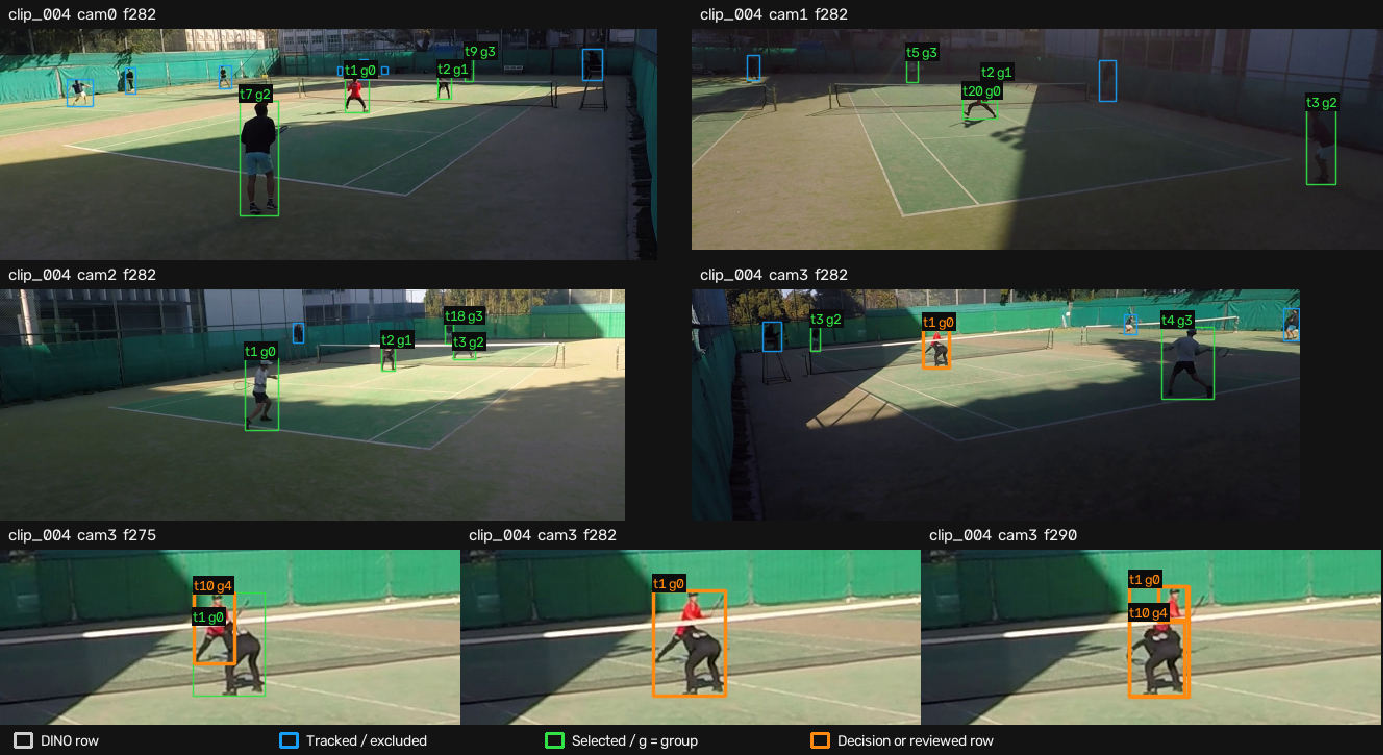
\includegraphics[width=\linewidth]{figures/players/clip_004-f0282.pdf}
\caption{clip\_004の元フレーム\ev{stopped-scenes}{282}の同期\ev{stopped-scenes}{4}視点と、cam3の前後。
cam3で重なった選手を同じboxが囲み、前後で追跡IDが交代した。
橙は診断対象、緑は選別済み、青は追跡済み・選別外、灰は追跡IDのない検出。}
\label{fig:stopped-004}
\end{figure}

\begin{figure}[tbp]
\centering
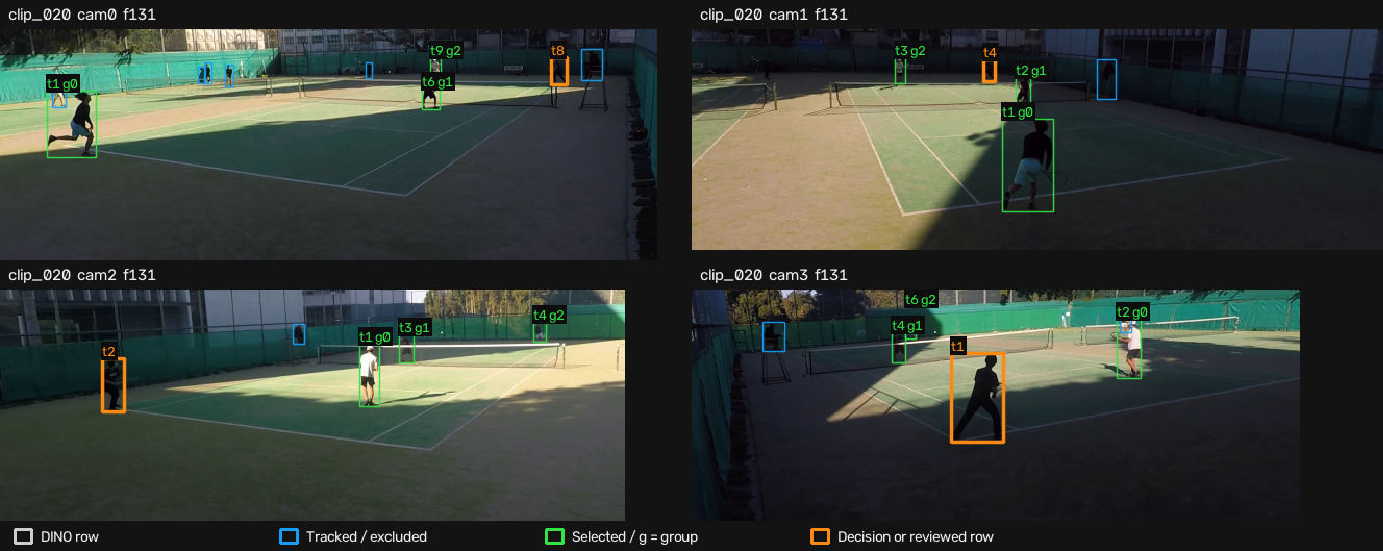
\includegraphics[width=\linewidth]{figures/players/clip_020-f0131.pdf}
\caption{clip\_020の元フレーム\ev{stopped-scenes}{131}の同期\ev{stopped-scenes}{4}視点。
不足した選手のboxとローカルIDが各視点に存在し、選別から外れていた。色は図\ref{fig:stopped-004}と同じ。}
\label{fig:stopped-020}
\end{figure}

保存特徴での再生は元の停止コードを\ev{stopped-replay}{14/14}件で再現した。
目視で確かめたDINO行の除去では\ev{stopped-replay}{0/8}件、同一選手と判断したグループの統合では\ev{stopped-replay}{0/2}件が回復した。
次点グループだけを外す感度比較では\ev{stopped-replay}{7/9}件が人物対応を通過し、
そのうち\ev{stopped-replay}{5}件で、レビューした時点の全選手が各\ev{stopped-replay}{2}視点以上に同じIDで残った。

\subsection{3Dで時間IDを決める選択経路}

現行の選択経路 \texttt{multiview\_3d\_tracking} は、全人物の2D関節から各時刻の3D骨格候補を作り、観測を排他的に割り当てる。
重なりや欠測をまたぐ時間窓で3D候補を結び、コート上の軌跡から選手を選別する。
複数視点の観測でカメラ内の途切れを補い、選手IDと対応する元検出行を身体復元へ渡す。

\begin{table}[tbp]
\centering
\caption{旧経路と3D時間追跡の比較。計測版は統合前の開発ブランチ。
4camでは同じ幾何と球を使い、全選手の身体復元・配置と球3Dを確認できたクリップを完了とした。
方式ごとに、関節の推定に使わなかった観測を採点し、クリップごとに再投影残差の中央値を求めた。}
\label{tab:tracking-3d}
\small
% Generated by scripts/make_tables.py.
\begin{tabular}{@{}lrr@{}}
\toprule
測定項目 & 旧経路 & 3D時間追跡 \\
\midrule
4cam 完了クリップ & \ev{track-3d-4cam}{52/69} & \ev{track-3d-4cam}{69/69} \\
4cam 全員の有効配置 [\%] & \ev{track-3d-4cam}{64.63} & \ev{track-3d-4cam}{90.74} \\
4cam 共通\ev{track-3d-4cam}{55}本の再投影中央値 [px] & \ev{track-3d-4cam}{7.89} & \ev{track-3d-4cam}{24.86} \\
3cam 予約未見のIDF1 [\%] & \ev{track-3d-3cam}{92.07} & \ev{track-3d-3cam}{80.42} \\
3cam 予約未見の選別再現率 [\%] & \ev{track-3d-3cam}{85.30} & \ev{track-3d-3cam}{67.25} \\
\bottomrule
\end{tabular}

\end{table}

Meiji 4camで完了は\ev{track-3d-4cam}{52/69→69/69}件に増え、選手再構成の停止は\ev{track-3d-4cam}{14→0}件に減った（表\ref{tab:tracking-3d}）。
予約未見のMeiji 3camでは射影した時間IDのIDF1が\ev{track-3d-3cam}{92.07→80.42\%}に下がった。
旧経路が校正で停止して新経路で補完した\ev{track-3d-3cam}{1}本を除いても、IDF1の低下が残った。
4camの共通クリップでは、再投影残差がクリップ中央値の中央値で\ev{track-3d-4cam}{7.89→24.86} pxへ増えた。
